%!TEX root = draft.tex
\vspace{-3.5mm}
\section{Queues With Fixed Dequeue Linearization Points}\label{sec:queues}
\vspace{-1.5mm}

The classical abstract queue implementation, denoted $AbsQ_0$, maintains a
sequence of enqueued values; dequeues return the oldest non-dequeued value, at
the time of their linearization points, or {\tt EMPTY}. Some implementations,
like the queue of \citet{journals/toplas/HerlihyW90}, denoted {\sc hwq} and
listed in Figure~\ref{fig:HerlihyWing}, are not forward-simulated by $AbsQ_0$,
even though they refine $AbsQ_0$, since the order in which their enqueues are
linearized to form $AbsQ_0$’s sequence is not determined until later, when their
values are dequeued.

\begin{figure}[t]
  \begin{minipage}[b]{0.55\linewidth}
    \begin{lstlisting}
void enq(int x) {
  i = back++; items[i] = x;
}
int deq() {
  while (1) {
    range = back - 1;
    for (int i = 0; i <= range; i++) {
      x = swap(items[i],null);
      if (x != null) return x;
} } }
    \end{lstlisting}
    \caption{The Herlihy \& Wing Queue~\cite{journals/toplas/HerlihyW90}.}
    \label{fig:HerlihyWing}

    \smallskip
    \hrule
    \smallskip

    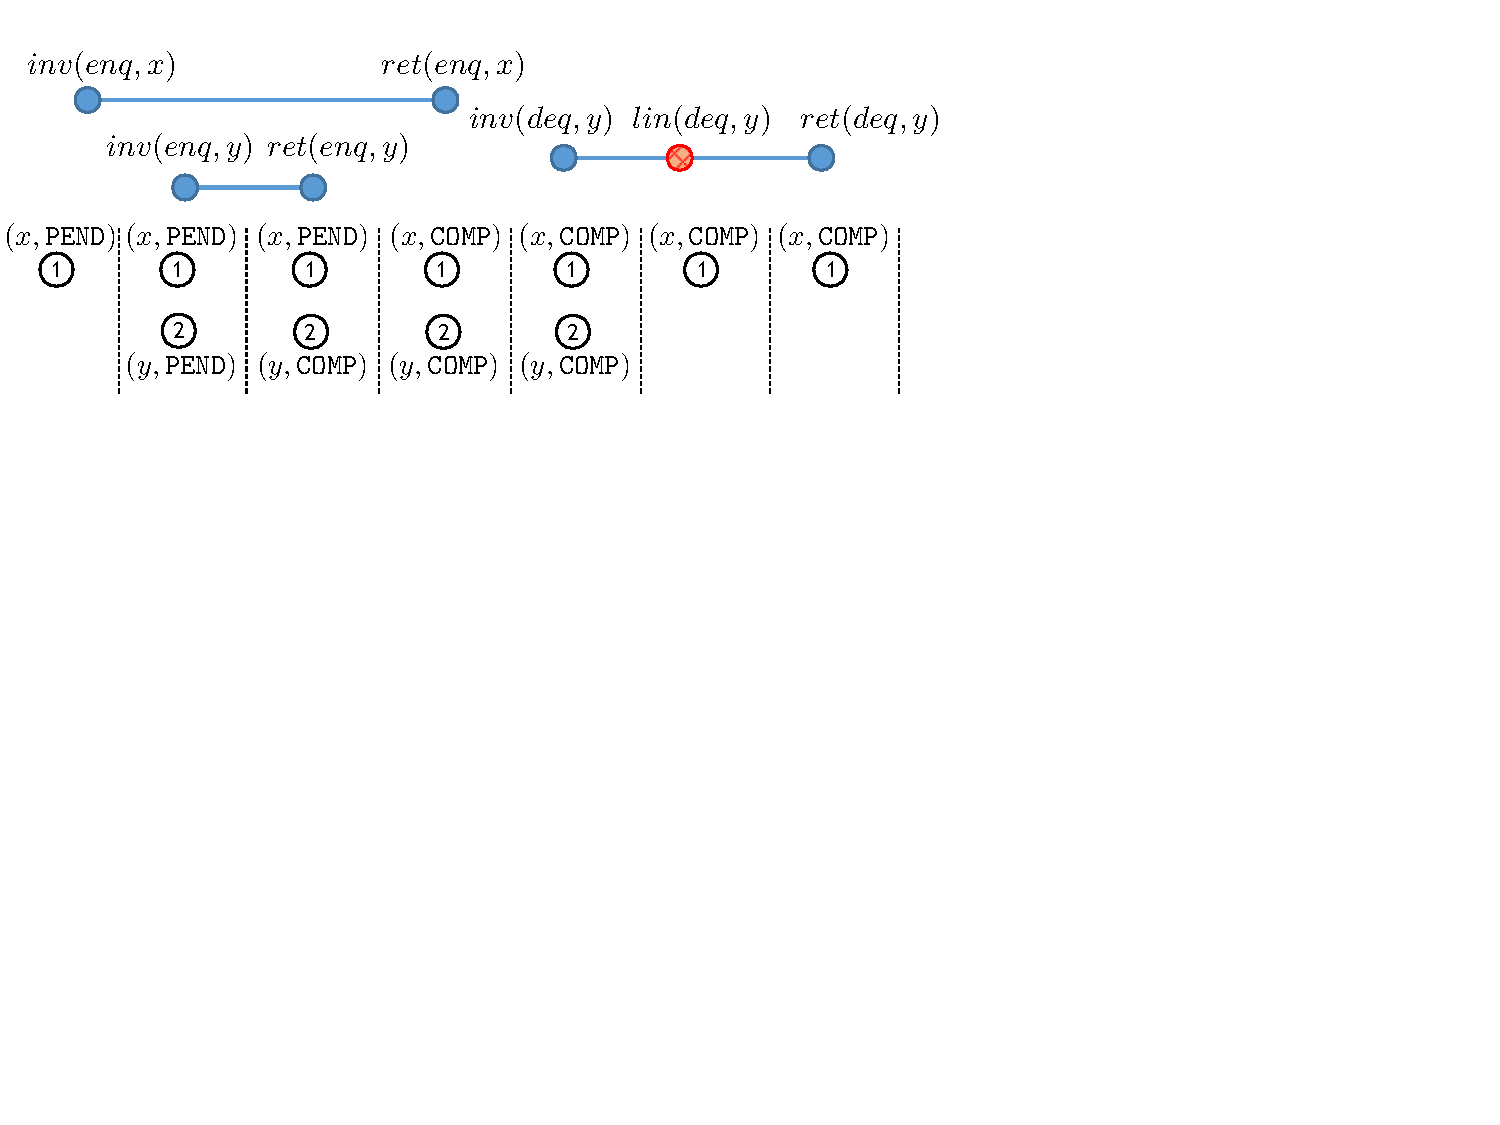
\includegraphics[width=7cm]{fig-queue1}
    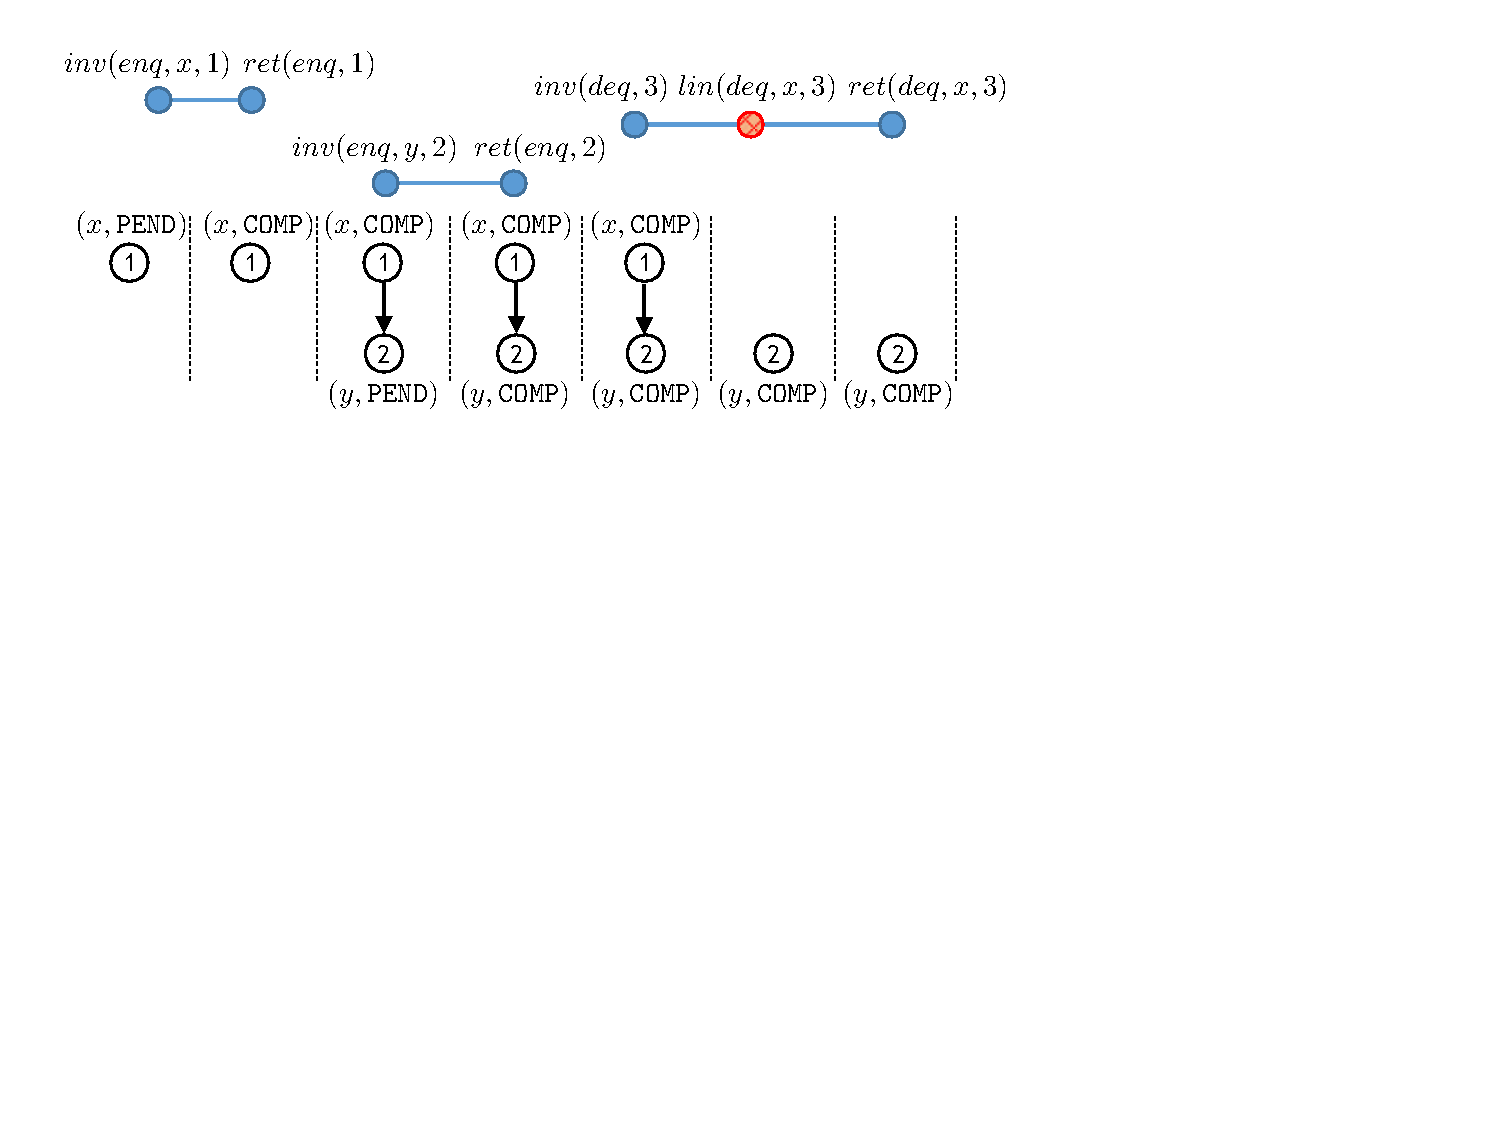
\includegraphics[width=7cm]{fig-queue2}
    \caption{Forward simulation with $AbsQ$. Lines depict operations,
    and circles depict call, return, and linearization point actions.}
    \label{fig:queueSim}
  \end{minipage}
  \hfill
  \begin{minipage}[b]{0.38\linewidth}
    \begin{lstlisting}
function loc: $\mathbb{O} \to \set{\tt inv, lin, ret, \bot}$
function arg, ret: $\mathbb{O} \to \mathbb{V}$
function present, pending: $\mathbb{O} \to \mathbb{B}$
function before: $\mathbb{O} \times \mathbb{O} \to \mathbb{B}$

rule inv(enq,v,k):
  arg(k) := v
  present(k) := true
  pending(k) := true
  forall k1 with present(k1):
    if $\lnot$pending(k1):
      before(k1,k) := true

rule ret(enq,k):
  pending(k) := false

rule inv(deq,k):
  pass

rule lin(deq,v,k):
  ret(k) := v
  if v = EMPTY:
    forall k' with present(k'):
      assert pending(k')
  else:
    let k1 = arg$^{-1}$(v)
    assert present(k1)
    forall k2 with present(k2):
      assert $\lnot$before(k2,k1)
    present(k1) := false

rule ret(deq,v,k):
  assert ret(k) = v
    \end{lstlisting}
    \caption{The $AbsQ$ implementation; each rule \lstinline|$\alpha$(\_,k)|
    implicitly begins with \lstinline|assert loc(k)=$\alpha$| and ends with
    the appropriate \lstinline|loc(k):=$\beta$|.}
    \label{fig:transitions:AbsQ}
  \end{minipage}
\end{figure}

In this section we develop an abstract queue implementation, denoted $AbsQ$,
which maintains a partial order of enqueues, rather than a linear sequence.
Since $AbsQ$ does not force refining implementations to eagerly pick among
linearizations of their enqueues, it forward-simulates many more queue
implementations. In fact, $AbsQ$ forward-simulates all queue implementations of
which we are aware that are not forward-simulated by $AbsQ_0$, including {\sc
hwq}, The Baskets Queue~\cite{DBLP:conf/opodis/HoffmanSS07}, The Linked
Concurrent Ring Queue ({\sc lcrq})~\cite{DBLP:conf/ppopp/MorrisonA13}, and The
Time-Stamped Queue~\cite{DBLP:conf/popl/DoddsHK15}.


%TODO HOW CAN WE CONVINCE THAT OTHER IMPLEMENTATIONS HAVE THE SAME PROPERTY ?
\vspace{-3.5mm}
\subsection{Enqueue Methods With Non-Fixed Linearization Points}
\vspace{-1mm}
% describe a queue implementation listed in Figure~\ref{fig:HerlihyWing} and known as the Herlihy \& Wing Queue~\cite{journals/toplas/HerlihyW90} ($\mathit{HWQ}$ for short), where only the dequeue methods have fixed linearization points.
We describe $\mathit{HWQ}$ where the linearization points of the enqueue methods are not fixed.
The shared state consists of an array {\tt items} storing the values in the queue and a counter {\tt back} storing the index of the first unused position in {\tt items}. Initially, all the positions in the array are {\tt null} and {\tt back} is 0.
An enqueue method starts by reserving a position in {\tt items} ({\tt i} stores the index of this position and {\tt back} is incremented so the same position can't be used by other enqueues) and then, stores the argument {\tt x} at this position. The dequeue method traverses the array {\tt items} starting from the beginning and atomically swaps {\tt null} with the encountered value. If the value is not {\tt null}, then the dequeue returns that value. If it reaches the end of the array, then it restarts.

The linearization points of the enqueues are not fixed, they depend on dequeues executing in the future. Consider the following trace with two concurrent enqueues (${\tt i}(k)$ represents the value of {\tt i} in operation $k$): $inv(enq,x,1)$, $inv(enq,y,2)$, ${\tt i}(1) = \mbox{{\tt bck++}}$, ${\tt i}(2) = \mbox{{\tt bck++}}$, ${\tt items[i(}2{\tt )]} = y$.
%\vspace{-1.5mm}
%\begin{align*}
%inv(enq,x,1)\ \ \ inv(enq,y,2)\ \ \ {\tt i}(1) = \mbox{{\tt bck++}}\ \ \ {\tt i}(2) = \mbox{{\tt bck++}}\ \ \ {\tt items[i(}2{\tt )]} = y
%\vspace{-1.5mm}
%\end{align*}
%\begin{align*}
%inv(enq,x,1)\ inv(enq,y,2)\ ({\tt i}_1 = 0,{\tt bck} = 1)\ ({\tt i}_2 = 1,{\tt bck} = 2)\ ({\tt items[1]} = y)
%\end{align*}
Assuming that the linearization point corresponds to the assignment of {\tt i}, the history of this trace should be linearized to $inv(enq,x,1)$, $ret(enq,1)$, $inv(enq,y,2)$, $ret(enq,2)$. However, a dequeue executing until completion after this trace will return $y$ (only position $1$ is filled in the array {\tt items}) which is not consistent with this linearization. On the other hand, assuming that enqueues should be linearized at the assignment of {\tt items[i]} and extending the trace with ${\tt items[i(}1{\tt )]} = x$ and a completed dequeue that in this case returns $x$, leads to the incorrect linearization: $inv(enq,y,2)$, $ret(enq,2)$, $inv(enq,x,1)$, $ret(enq,1)$, $inv(deq,3)$, $ret(deq,x,3)$.
%\vspace{-1.5mm}
%\begin{align*}
%inv(enq,y,2)\ ret(enq,2) inv(enq,x,1)\ ret(enq,1)\ inv(deq,3)\ ret(deq,x,3).
%\vspace{-1.5mm}
%\end{align*}

The dequeue method has a fixed linearization point which corresponds to an execution of {\tt swap} returning a non-null value. This action alone contributes to the effect of that value being removed from the queue. Every concurrent history can be linearized to a sequential history where dequeues occur in the order of their linearization points in the concurrent history.
This claim is formally proved in Section~\ref{ssec:HerlihyWing}.

Since the linearization points of the enqueues are determined by future dequeue invocations, there exists no forward simulation from $\mathit{HWQ}$ to $AbsQ_0$.
In the following, we describe the abstract implementation $AbsQ$ for which such a forward simulation does exist.

\vspace{-3.5mm}
\subsection{Abstract Queue Implementation}
\vspace{-1.5mm}

%\textcolor{red}{Important: I think EMPTY return is problematic and I defined it wrong in my machine too. We should be able to return EMPTY if there are only pending nodes. Consider the following history of $AbsQ_0$: $inv(enq, d_1,k_1), inv(enq, d_2,k_2), inv(deq, k_3), lin(deq, \texttt{EMPTY}, k_3)$. This history should be reflected in $AbsQ$ by enabling lin \texttt{EMPTY} of dequeue when there are pending nodes. We also need to update the rules in figure.}
Informally, $AbsQ$ records the set of enqueue operations, whose argument has not yet been removed by a matching dequeue operation. In addition, it records the happens-before order between those enqueue operations: this is a partial order ordering an enqueue $k_1$ before another enqueue $k_2$ iff $k_1$ returned before $k_2$ was invoked.
%Informally, $AbsQ$ records the happens-before order between enqueue operations for which the added value has not been removed by a dequeue operation.
The linearization point of a dequeue can either remove a minimal enqueue $k$ (w.r.t. the happens-before stored in the state) and fix the return value to the value $d$ added by $k$, or fix the return value to ${\tt EMPTY}$ provided that the current state stores only pending enqueues (intuitively, the dequeue overlaps with all the enqueue operations stored in the current state and it can be linearized before all of them).
%with return value $d\neq{\tt EMPTY}$ is enabled only if the happens-before stored in the current state contains a minimal enqueue that adds the value $d$. The effect of the linearization point is that the minimal enqueue is removed from the current state and the return value is recorded in the library state.
%When
%%\noindent
%the return value is {\tt EMPTY}, the linearization point of a dequeue is enabled only if the current state stores only pending enqueues (because, the dequeue overlaps with all the enqueue operations stored in the current state and it can be linearized before all of them).
%The return of a dequeue is enabled only if the returned value matches the one fixed at the linearization point.

Fig.~\ref{fig:queueSim} pictures two executions of $AbsQ$ for two extended histories (that include dequeue linearization points). The state of $AbsQ$ after each action is pictured as a graph below the action. The nodes of this graph represent enqueue operations and the edges happens-before constraints. Each node is labeled by a value (the argument of the enqueue) and a flag {\tt PEND} or {\tt COMP} showing whether the operation is pending or completed. For instance, in the case of the first history, the dequeue linearization point $lin(deq,y,3)$ is enabled because the current happens-before contains a \emph{minimal} enqueue operation with argument $y$. Note that a linearization point $lin(deq,x,3)$ is also enabled at this state.

For readability, we define $AbsQ$ as an abstract state machine, which is given in Fig.~\ref{fig:transitions:AbsQ}. The shared state of $AbsQ$ consists of several boolean predicates indicating whether the value added by an enqueue has not been removed yet (the predicate $\mathsf{present})$, whether an enqueue is pending (the predicate $\mathsf{pending}$), the happens-before order (the predicate $\mathsf{before}$), and a function giving the value added by an enqueue (the function $\mathsf{arg}$). In the initial state, the domain of every function (predicate) is empty.
%the states of $AbsQ$ are tuples $\tup{O,<,\ell,rv,cp}$ where $O\subseteq \<Ops>$ is a set of operation identifiers, $<\subseteq O\times O$ is a strict partial order, $\ell: O -> \<Vals>\times\{\tt{PEND,\tt{COMP}}\}$ labels every identifier with a value and a pending/completed flag (the flag is used to track the happens-before order), $rv:\<Ops> ~> \<Vals>$ records the return value of a dequeue fixed at its linearization point ($~>$ denotes a partial function), and $cp:\<Ops> ~> \{A_1,A_2,R_1,R_2,R_3\}$ records the control point of every enqueue ($A_1, A_2$) or dequeue operation ($R_1,R_2,R_3$).
%All the components are $\emptyset$ in the initial state, and the transition relation $->$ is defined in Fig.~\ref{fig:transitions:AbsQ}. The alphabet of $AbsQ$ contains call/return actions and dequeue linearization points, denoted by $lin(deq,d,k)$. $Lin(deq)$ is the set of all actions $lin(deq,d,k)$.
%
The enqueue operations consist of two macro rules: the rule {\tt inv(enq,x,k)} orders the invoked operation after all the completed enqueues present in the current state ({\tt k} is a fresh operation identifier associated to the current operation), and the rule {\tt ret(enq,k)} sets $\mathsf{pending}${\tt (k)} to {\tt false}. % provided that the operation is still present in the current state.
The dequeue operations consist of two rules {\tt inv(deq,k)} and {\tt ret(deq,y,k)} associated to the invocation and respectively, the return action, whose definition is obvious, and the rule {\tt lin(deq,y,k)} corresponding to its linearization point. When a non-empty set of pending enqueues are present, the rule {\tt lin(deq,y,k)} is non-deterministic. It can set the return value {\tt y} either to {\tt EMPTY}, or to a value {\tt d} $\neq$ {\tt EMPTY}, provided that {\tt d} has been added by an enqueue {\tt k1} which is minimal in the current happens-before. In the latter case, $\mathsf{present}${\tt (k1)} is set to {\tt false} to indicate that {\tt k1}'s argument has been removed. When there exists at least one completed enqueue whose value has not been removed, the rule {\tt lin(deq,y,k)} sets {\tt y} to the value added by a minimal enqueue (w.r.t. the current happens-before).

%{\sc call-enq} orders the invoked operation after all the completed enqueues in the current state, and the rules {\sc ret-enq1}/{\sc ret-enq2} flip the corresponding flag from {\tt PEND} to {\tt COMP} provided that the operation is still present in the current state. For dequeue operations, {\sc call-deq} only increments the control point and {\sc ret-deq} checks whether the return value is the same as the one fixed at the linearization point. The linearization point rule {\sc lin-deq1} corresponds to the case of a non-empty queue, showing that $lin(deq,d,k)$ is enabled only if $d$ has been added by an enqueue which is minimal in the current happens-before. When enabled, it removes the enqueue adding $d$ from the state. The linearization point rule {\sc lin-deq2} corresponds to the case of dequeue operations linearized with an {\tt EMPTY} return value.


% Let $AbsQ_0$ denote this implementation (formally defined in Appendix~\ref{app:absImplQueue}).
The following result states that the library $AbsQ$ has exactly the same set of histories as the standard abstract library $AbsQ_0$. % (see Appendix~\ref{app:absImplQueue} for a proof).

\vspace{-1.5mm}
\begin{theorem}\label{th:absImplQueue}
$AbsQ$ is a refinement of $AbsQ_0$ and vice-versa.
\vspace{-2mm}
\end{theorem}

The abstract state machine in Fig.~\ref{fig:transitions:AbsQ} defines an LTS over the alphabet $C\cup R\cup Lin(deq)$. The transitions corresponding to the rule {\tt lin(deq,y,k)} are labeled by  actions $lin(deq,y,k)$. Also, we assume that the transition corresponding to the invocation of a method is done atomically with the first step of the same invocation (the macro rule {\tt inv(...)}), and similarly for transitions corresponding to returning from a method, they are done atomically with the last step (the macro rule {\tt ret(...)}). They are labeled as expected with call/return actions (borrowing the operation identifier which occurs as argument of the macro rules). It can be easily proved that this assumption doesn't modify the set of traces projected on $C\cup R\cup Lin(deq)$ (compared to an LTS where these steps are not atomic).

%~\footnote{Without this assumption, while proving forward simulations, a call/return action in the concrete implementation is simulated by two steps of the abstract implementation, the call/return action together with the first/last macro rule.}.


A trace of a queue implementation is called \emph{$Lin(deq)$-complete} when every completed dequeue has a linearization point, i.e., each return action $ret(deq,d,k)$ is preceded by an action $lin(deq,d,k)$. A queue implementation $L$ over alphabet $\Sigma$, such that $C\cup R\cup Lin(deq)\subseteq \Sigma$, is called \emph{with fixed dequeue linearization points} when every trace $@t\in Tr(L)$ is $Lin(deq)$-complete.

%TODO NEEDS DATA INDEPENDENCE FOR THE LINEARIZATION POINT TRANSITIONS TO BE DETERMINISTIC

The following result shows that $C\cup R\cup Lin(deq)$-forward simulations are a sound and complete proof method for showing the correctness of a queue implementation with fixed dequeue linearization points (up to the correctness of the linearization points). It is obtained from Theorem~\ref{th:absImplQueue} and Theorem~\ref{th:forSim} using the fact that the alphabet of $AbsQ$ is exactly $C\cup R\cup Lin(deq)$ and $AbsQ$ is deterministic. The determinism of $AbsQ$ relies on the assumption that every value is added at most once. Without this assumption, $AbsQ$ may reach a state with two enqueues adding the same value being both minimal in the happens-before. A transition corresponding to the linearization point of a dequeue from this state can remove any of these two enqueues leading to two different states. Therefore, $AbsQ$ becomes non-deterministic. Note that this is independent of the fact that $AbsQ$ manipulates  operation identifiers.

\vspace{-1.5mm}
\begin{corollary}
A queue implementation $L$ with fixed dequeue linearization points is a $C\cup R\cup Lin(deq)$-refinement of $AbsQ_0$ if{f} there exists a $C\cup R\cup Lin(deq)$-forward simulation from $L$ to $AbsQ$.
\vspace{-1.5mm}
\end{corollary}

\vspace{-4.5mm}
\subsection{A Correctness Proof For Herlihy\&Wing Queue}\label{ssec:HerlihyWing}
\vspace{-1mm}
We describe a forward simulation $F_1$ from $\mathit{HWQ}$ to $AbsQ$. The description of $\mathit{HWQ}$ in Fig.~\ref{fig:HerlihyWing} defines an LTS whose states contain the shared array ${\tt items}$ and the shared counter ${\tt back}$ together with a valuation for the local variables ${\tt i}$, ${\tt x}$, and ${\tt range}$, and the control location of each operation. A transition is either a call or a return action, or a statement in one of the two methods ${\tt enq}$ or ${\tt deq}$.

%An enqueue operation in a $\mathit{HWQ}$ state is pending and present if and only if its argument is stored in the array ${\tt items}$ or it has not yet written to the array  ${\tt items}$. Those operations should be $\mathsf{pending}$ and $\mathsf{present}$ in the related $AbsQ$ states. In addition to this, the forward simulation $F_1$ imposes following restrictions:
An $\mathit{HWQ}$ state $s$ is related by $F_1$ to $AbsQ$ states $t$ where the predicate
$\mathsf{present}$ is true for all the enqueues in $s$ whose argument is stored in the array ${\tt items}$, and all the pending enqueues that have not yet written to the array ${\tt items}$ (and only for these enqueues). We refer to such enqueues in $s$ as $\mathsf{present}$ enqueues. Also, $\mathsf{pending}(k)$ is ${\tt true}$ in $t$ whenever $k$ is a pending enqueue in $s$, $\mathsf{arg}(d)=k$ in $t$ whenever the argument of the enqueue $k$ in $s$ is $d$, and for every dequeue operation $k$ such that ${\tt x}(k)=d\neq {\tt null}$, we have that ${\tt y}(k)=d$ (recall that ${\tt y}$ is a local variable of the dequeue method in $AbsQ$). The order relation $\mathsf{before}$ in $t$ satisfies the following constraints:
\vspace{-2mm}
\begin{itemize}
	\item[(a)] pending enqueues are maximal, i.e., for every two $\mathsf{present}$ enqueues $k$ and $k'$ such that $k'$ is $\mathsf{pending}$, we have that $\neg \mathsf{before}(k',k)$, % $k'\not< k$,
	\item[(b)] $\mathsf{before}$ is consistent with the order in which positions of ${\tt items}$ have been reserved, i.e., for every two present enqueues $k$ and $k'$ such that ${\tt i}(k) < {\tt i}(k')$, we have that $\neg \mathsf{before}(k',k)$, %$k' \not< k$,
	\item[(c)] if the position $i$ reserved by an enqueue $k$ has been ``observed'' by a non-linearized dequeue that in the current array traversal may ``observe'' a later position $j$ reserved by another enqueue $k'$, then $k$ can't be ordered before $k'$,
%	an enqueue which has reserved a position $i$ %and executed only the first statement
%	can't be ordered before another enqueue that has reserved a position $j \geq i$ ,
	i.e., for every two present enqueues $k$ and $k'$, and a dequeue $k_d$, such that

	\vspace{-2mm}
	\noindent
	{\small
	\begin{align}
	\hspace{-8mm}
	{\tt canRemove}(k_d,k') \land ({\tt i}(k) < {\tt i}(k_d) \lor ({\tt i}(k)={\tt i}(k_d) \land {\tt afterSwapNull}(k_d)))
\label{eq:inst}
	\end{align}}

	\vspace{-6mm}
	\noindent
	we have that $\neg \mathsf{before}(k,k')$. The predicate ${\tt canRemove}(k_d,k')$ holds when $k_d$ visited a {\tt null} item in {\tt items} and the position $i(k')$ reserved by $k'$ is in the range of $(k_d)$ i.e., $({\tt x}(k_d) = {\tt null} \land {\tt i}(k_d) < {\tt i}(k') \leq {\tt range}(k_d)) \lor ({\tt i}(k_d) = {\tt i}(k') \land {\tt beforeSwap}(k_d) \land {\tt items}[{\tt i}(k')] != {\tt null})$. The predicate ${\tt afterSwapNull}(k_d)$ (resp., ${\tt beforeSwap}(k_d)$) holds when the dequeue $k_d$ is at the control point after a ${\tt swap}$ returning ${\tt null}$ (resp., before a ${\tt swap}$).
\vspace{-2mm}
\end{itemize}
%\noindent
%An enqueue is labeled by $(d,{\tt PEND})$ where $d$ is the input value if it's pending and by  $(d,{\tt COMP})$, otherwise.
%The constraint (a) ensures  on $\mathsf{before}$ ensure that: (i) every present and pending enqueue is maximal  and (ii) a present enqueue whose argument is about to be removed by a dequeue operation is minimal.
%
%The first point is ensured by the constraint (a).
%%Present and pending enqueue identifiers in the $\mathit{HWQ}$ state are $\mathsf{pending}$ in the related $AbsQ$ state and $\mathsf{pending}$ enqueues are maximal in a valid $AbsQ$ state.
%
The constraints on $\mathsf{before}$ ensure that a present enqueue whose argument is about to be removed by a dequeue operation is minimal. Thus, let $k'$ be a present enqueue that inserted its argument to ${\tt items}$, and $k_d$ a pending dequeue such that ${\tt canRemove}(k_d, k')$ holds and $k_d$ is just before its swap action at the reserved position of $k'$ i.e., ${\tt i}(k_d) = {\tt i}(k')$. Another pending enqueue $k$ cannot be ordered before $k'$ since pending enqueues are maximal by (a). Regarding the completed and present enqueues $k$, we consider two cases: $i(k) > i(k')$ and $i(k) < i(k')$. For the former case, the constraint (b) ensures $\neg \mathsf{before}(k,k')$ and for the latter case the constraint (c) ensures $\neg \mathsf{before}(k,k')$. Consequently, $k'$ is a minimal element w.r.t. $\mathsf{before}$ just before $k_d$ removes its argument.

Next, we show that $F_1$ is indeed a $C\cup R\cup Lin(deq)$-forward simulation. Let $s$ and $t$ be states of $\mathit{HWQ}$ and $AbsQ$, respectively, such that $(s,t)\in F_1$.
We omit discussing the trivial case of transitions labeled by call and return actions which are simulated by similar transitions of $AbsQ$. % (for the return a dequeue operation $k$, we use the equality between the local variable ${\tt x}(k)$ in $s$ and the component $rv(k)$ in $t$).
%\textcolor{red}{ I think it is good to mention again that call/return actions in HWQ correspond to the same call/return actions in AbsQ (without any other internal action). I also think that invoke enqueue operation is non-trivial. Preservation of the strict partial order and all of the above items a, b and c needs to be rechecked.}

%\setlength{\parskip}{0pt}
We show that each internal step of an enqueue or dequeue, except a {\tt swap} returning a non-null value in dequeue (which represents its linearization point), is simulated by an \emph{empty} sequence of $AbsQ$ transitions, i.e., for every state $s'$ obtained through one of these steps, if $(s,t)\in F_1$, then $(s',t)\in F_1$ for each $AbsQ$ state $t$.
Essentially, this consists in proving the following property, called \emph{monotonicity}: the set of possible $\mathsf{before}$ relations associated by $F_1$ to $s'$ doesn't exclude any order $\mathsf{before}$ associated to $s$.
%Essentially, this boils down to showing that the constraints over $<$ in the definition of $\mathit{fs}$ are an invariant for these steps.

Concerning enqueue rules, let $s'$ be the state obtained from $s$ when a pending enqueue $k$ reserves an array position. This enqueue must be maximal in both $t$ and any state $t'$ related to $s'$ (since it's pending). Moreover, there is no dequeue that can ``observe'' this position before restarting the array traversal. Therefore, item (c) in the definition of $F_1$ doesn't constrain the order between $k$ and some other enqueue neither in $s$ nor in $s'$. Since this transition doesn't affect the constraints on the order between enqueues different from $k$ (their local variables remain unchanged), monotonicity holds. This property is trivially satisfied by the second step of enqueue which doesn't affect {\tt i}.

To prove monotonicity in the case of dequeue internal steps different from its linearization point, it is important to track the non-trivial instantiations of item (c) in the definition of $\mathsf{before}$ over the two states $s$ and $s'$, i.e., the triples $(k,k',k_d)$ for which (\ref{eq:inst}) holds. Instantiations that are enabled only in $s'$ may in principle lead to a violation of monotonicity (since they restrict the orders $\mathsf{before}$ associated to $s'$). For the two steps that begin an array traversal, i.e., reading the index of the last used position and setting {\tt i} to $0$, there exist no  such new instantiations in $s'$ because the value of {\tt i} is either not set or $0$. % (it is trivial to notice that applying these steps doesn't disable such instantiations that were possible in $s$).
%The same holds for the step incrementing the iterator {\tt i}.
%
%The execution of {\tt swap} returning {\tt null} may introduce one new non-trivial instantiation $(k,k',k_d)$ of item (c).
%We write ${\tt i}_s(k)$ to refer to the value of the variable {\tt i} of operation $k$ in state $s$. Assume that indeed, there exist two enqueue operations $k$ and $k'$ such that ${\tt i}_{s'}(k) < {\tt i}_{s'}(k_d) \leq {\tt i}_{s'}(k')$, ${\tt x}_{s'}(k_d)={\tt null}$, ${\tt i}_{s'}(k') \leq {\tt range}_{s'}(k_d)$ TODO SWAP. Since {\tt swap} returnes {\tt null}, the position ${\tt i}_{s'}(k_d)$
%
%
% and ${\tt i}_{s}(k) = {\tt i}_{s'}(k_d)$. The latter constraint guarantees that this instantiation is not enabled in state $s$. The increment of {\tt i} being enabled, implies that
%
The same is true for the increment of {\tt i} in a dequeue $k_d$ since the predicate ${\tt afterSwapNull}(k_d)$ holds in state $s$.
The execution of {\tt swap} returning {\tt null} in a dequeue $k_d$ enables new instantiations $(k,k',k_d)$ in $s'$, thus adding potentially new constraints $\neg \mathsf{before}(k,k')$. We show that these instantiations are however vacuous because $k$ must be pending in $s$ and thus maximal in every order $\mathsf{before}$ associated by $F_1$ to $s$.
Let $k$ and $k'$ be two enqueues such that together with the dequeue $k_d$ they satisfy the property (\ref{eq:inst}) in $s'$ but not in $s$.
We write ${\tt i}_s(k)$ for the value of the variable {\tt i} of operation $k$ in state $s$.
We have that ${\tt i}_{s'}(k) = {\tt i}_{s'}(k_d) \leq {\tt i}_{s'}(k')$ and ${\tt items}[{\tt i}_{s'}(k_d)]={\tt null}$. The latter implies that the enqueue $k$ didn't execute
the second statement (since the position it reserved is still {\tt null}) and it is pending in $s'$. The step that swaps the null item does not modify anything except the control point of $k_d$ that makes ${\tt afterSwapNull}(k_d)$ true in $s'$ . Hence, $i_s(k) = i_s(k_d)\leq i_s(k')$ and ${\tt items}[i_s(k_d)] = {\tt null}$ is also true. Therefore, $k$ is pending in $s$ and maximal. Hence, $\mathsf{before}(k,k')$ is not true in both $s$ and $s'$.

Finally, we show that the linearization point of a dequeue $k$ of $\mathit{HWQ}$, i.e., an execution of {\tt swap} returning a non-null value $d$, from state $s$ and leading to a state $s'$ is simulated by a transition labeled by $lin(deq,d,k)$ of $AbsQ$ from state $t$. By the definition of $\mathit{HWQ}$, there is a unique enqueue $k_e$ which filled the position updated by $k$, i.e., ${\tt i}_s(k_e)=i_s(k)$ and ${\tt x}_{s'}(k)={\tt x}_s(k_e)$.

We show that $k_e$ is minimal in the order $\mathsf{before}$ of $t$ which implies that $k_e$ could be chosen by $lin(deq,d,k)$ step applied on $t$. As explained previously, instantiating item (c) in the definition of $\mathsf{before}$ with $k'=k_e$ and $k_d=k$, and instantiating item (b) with $k=k_e$, we ensure the minimality of $k_e$. Moreover, the state $t'$ obtained from $t$ through a $lin(deq,d,k)$ transition is related to $s'$ because the value added by $k_e$ is not anymore present in {\tt items} and $\mathsf{present}(k_e)$ doesn't hold in $t'$.
%Thus, instantiating item (c) in the definition of $\mathsf{before}$ with $k'=k_e$ and $k_d=k$ we get that every enqueue that reserved a position smaller than the one of $k_e$ can't be ordered before $k_e$ in the order $\mathsf{before}$. Also, applying item (b) with $k=k_e$ we get the same for every enqueue that reserved a bigger position. An enqueue that didn't reserve a position is by definition maximal in $<$ and therefore, not a predecessor of $k_e$. Then, the state $t'$ obtained from $t$ through a $lin(deq,d,k)$ transition is related to $s'$ because (1) the value added by $k_e$ is not anymore present in {\tt items} which implies that $k_e$ doesn't occur in any $AbsQ$ state related to $s'$, and (2) the value of ${\tt x}(k)$ is set to $d\neq {\tt null}$ which implies that $rv(k)$ is set to $d$ in every $AbsQ$ state related to $s'$.
%
%\vfill
%
